\section{算子列的收敛}
\label{sec:lop-operator-convergence}

实际计算中，我们常用一列逐渐精细的近似算子$T_n$代替一个算子$T$，例如只保留前$n$个展开系数，或者把积分区域截去一小块。对手中的每个输入，近似输出会越来越准；但这是否意味着存在一个只依赖$n$的误差界，对所有单位输入同时有效？

有限维中这不成问题：矩阵的每个元素收敛，整个矩阵就按任何范数收敛。无限维中矩阵有无穷多列，“每一列都收敛”和“所有列一起收敛”不再是一回事，这两种要求的量词次序不同，强弱也不同。

\begin{definition}[算子范数收敛与强算子收敛]
\label{def:lop-operator-convergence}
设$X,Y$是赋范空间，$T_n,T\in\mathcal B(X,Y)$。若
\begin{equation}
 \lVert T_n-T\rVert\to0,
 \label{eq:lop-norm-convergence}
\end{equation}
则称$T_n$\term{算子范数收敛}（convergence in operator norm）到$T$。若
\begin{equation}
 \lVert T_nx-Tx\rVert_Y\to0\qquad(\text{对每个}x\in X),
 \label{eq:lop-strong-convergence}
\end{equation}
则称$T_n$\term{强算子收敛}（strong operator convergence）到$T$。
\end{definition}

算子范数收敛给出统一误差：$\lVert T_n-T\rVert$只依赖$n$，对单位球中的全部输入同时控制输出误差。强算子收敛给出逐输入误差：先固定$x$，再让$n\to\infty$，收敛快慢可以随$x$变化。由
\[
 \lVert T_nx-Tx\rVert\leq\lVert T_n-T\rVert\,\lVert x\rVert,
\]
算子范数收敛蕴含强算子收敛；下面的例子说明反过来不成立。

强算子收敛中的“逐点”，指的是对每个输入向量$x$，像向量$T_nx$在$Y$的范数下收敛。当$X,Y$是函数空间时，它不是说函数$T_nx$在定义域的每个点处收敛，后者是函数列的另一种收敛方式，二者不能混用。

\paragraph{截断投影}
设$H$是无限维可分Hilbert空间，$(e_k)_{k\geq1}$是标准正交基，$P_n$是到$\operatorname{span}\{e_1,\ldots,e_n\}$的正交投影，即
\[
 P_nx=\sum_{k\leq n}\langle e_k,x\rangle e_k.
\]
按第~\ref{sec:lop-norm-definition}小节的矩阵表示，$P_n$是对角矩阵$\operatorname{diag}(1,\ldots,1,0,0,\ldots)$，前$n$个对角元素为$1$。

固定$x$。由第~\ref{chap:function-inner-product-spaces}章的Parseval等式，
\[
 \lVert x-P_nx\rVert^2=\sum_{k>n}\lvert\langle e_k,x\rangle\rvert^2\to0,
\]
因为右端是一个收敛级数的尾部，这个级数的和是$\lVert x\rVert^2$。所以$P_n$强算子收敛到恒等算子$I$。

另一方面，对每个$n$，被截掉的单位向量$e_{n+1}$满足$P_ne_{n+1}=0$，于是
\[
 \lVert(I-P_n)e_{n+1}\rVert=1.
\]
又$I-P_n$是到正交补的投影，$\lVert I-P_n\rVert\leq1$。所以$\lVert I-P_n\rVert=1$对一切$n$成立，$P_n$不按算子范数收敛到$I$。在矩阵上看，差$I-P_n$是$\operatorname{diag}(0,\ldots,0,1,1,\ldots)$，对角线上总还有$1$。

图~\ref{fig:lop-projection-strong-norm}比较了三个输入的截断误差。系数为$2^{-k/2}$的单位向量，其截断误差为$2^{-n/2}$，衰减很快；系数与$1/k$成比例的单位向量衰减慢得多。

\begin{BookInlineFigure}
  \centering
  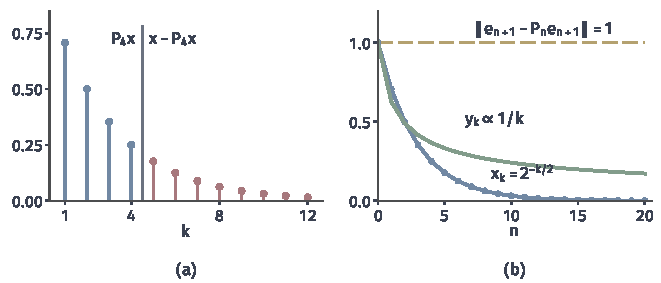
\includegraphics[width=112mm]{figures/04-spaces-measures-and-geometry/03-function-spaces/matplotlib/lop-projection-strong-norm/figure.pdf}
  \caption{截断投影的强收敛与算子范数不收敛。(a)单位向量$x$的系数$c_k=2^{-k/2}$，$P_4$保留蓝色的前四项，红色尾项构成误差$x-P_4x$。(b)截断误差随保留项数$n$的变化：$\lVert x-P_nx\rVert=2^{-n/2}$（蓝），系数与$1/k$成比例的单位向量$y$（绿）衰减较慢，而被截掉的基向量$e_{n+1}$的误差始终为$1$（黄虚线）。}
  \label{fig:lop-projection-strong-norm}
\end{BookInlineFigure}

每个固定输入的误差都趋于零，但不同输入的速度可以任意慢，而被截掉的那个基向量的误差始终是$1$。“每个元素都能被有限维子空间逼近”并不意味着同一个有限维子空间能以任意精度统一逼近整个单位球。

\paragraph{有限个输入上的统一控制}
强算子收敛对有限个输入仍可同时控制。设$x^{(1)},\ldots,x^{(m)}$是固定的输入，对每个$i$取$N_i$使误差小于$\varepsilon$，再取$N=\max_iN_i$即可。

截断投影失去统一控制的原因是单位球中有无穷多个相互正交的方向，每个$P_n$只能照顾其中有限个。第~\ref{sec:lop-uniform-boundedness}小节将说明，在Banach空间上，强算子收敛的算子列至少有统一的范数上界。

\paragraph{函数空间中的截断}
在$L^2(0,1)$中，按二分区间依次排列
\[
 I_1=[0,1],\quad I_2=[0,\tfrac12],\quad I_3=[\tfrac12,1],\quad I_4=[0,\tfrac14],\ \ldots,
\]
长度$\lvert I_n\rvert\to0$。令$T_nf=(1-\mathbf 1_{I_n})f$，即把输入在$I_n$上的部分抹去，这是一个乘法算子。对每个$f\in L^2$，
\[
 \lVert f-T_nf\rVert_2^2=\int_{I_n}\lvert f\rvert^2\,\mathrm dx\to0,
\]
因为$\lvert f\rvert^2$可积，积分区域的测度趋于零时积分趋于零。所以$T_n$强算子收敛到$I$。

同一列算子却不按算子范数收敛。取$f_n=\lvert I_n\rvert^{-1/2}\mathbf 1_{I_n}$，它是单位向量且$(I-T_n)f_n=f_n$，故$\lVert I-T_n\rVert=1$。

更值得注意的是，取$f=1$，每个$x\in[0,1]$都落在无穷多个$I_n$中，也落在无穷多个$I_n$之外。于是$(T_nf)(x)$在$0$与$1$之间无穷次跳动，对任何$x$都不收敛。强算子收敛成立，输出函数却在每一点都不收敛，这正说明二者是不同的概念。
